% This is samplepaper.tex, a sample chapter demonstrating the
% LLNCS macro package for Springer Computer Science proceedings;
% Version 2.20 of 2017/10/04
%
\documentclass[runningheads]{llncs}
%
\usepackage{graphicx}
\usepackage{amssymb}
\usepackage{amsmath}
\usepackage{siunitx}
\usepackage{booktabs}
\usepackage{float}
\usepackage[spanish]{babel}
\usepackage[utf8]{inputenc}
\usepackage[T1]{fontenc}
\usepackage{hyperref}

% Used for displaying a sample figure. If possible, figure files should
% be included in EPS format.
%
% If you use the hyperref package, please uncomment the following line
% to display URLs in blue roman font according to Springer's eBook style:
% \renewcommand\UrlFont{\color{blue}\rmfamily}

\begin{document}

\title{EasyCript, una herramienta para pruebas criptográficas}
%If Title is too long, use \titlerunning
%\titlerunning{Short Title}

%Single insitute
\author{Diego Lupi, Pedro Nieto, Huaira Gómez}
%If there are too many authors, use \authorrunning
%\authorrunning{First Author et al.}
\institute{FaMAF - Universidad Nacional de Córdoba, Córdoba, Argentina}


%% Multiple insitutes - ALTERNATIVE to the above
% \author{%
%     Firstname Lastname\inst{1} \and
%     Firstname Lastname\inst{2}
% }
%
%If there are too many authors, use \authorrunning
%  \authorrunning{First Author et al.}
%
%  \institute{
%      Insitute 1\\
%      \email{...}\and
%      Insitute 2\\
%      \email{...}
%}

\maketitle

\begin{abstract}
Easycrypt\cite{ref_article1} es una herramienta automatizada que soporta la construcción y verificación de pruebas de seguridad de sistemas criptográficos. Permite mejorar la confianza en los mismos mediante la entrega de pruebas verificadas formalmente que resultan en sus metas propuestas. Provee una plataforma versátil que soporta pruebas automatizadas pero también permite al usuario realizar pruebas complejas de manera interactiva entrelazando la verificación del programa con la formalización de las matemáticas, hecho fundamental al formalizar pruebas criptográficas. Con este paper nos proponemos mostrar las características de esta herramienta y compararla con herramientas similares.

\keywords{Easycrypt  \and Game-based cryptographic proofs \and Probabilistic.}
\end{abstract}
%
%
%
\section{Introducción}
Desde siempre las pruebas criptográficas fueron propensas a errores, lo que naturalmente las puede llevar a ser incorrectas.
 En particular en las pruebas de seguridad criptográficas la correctitud es crítica para mejorar la confianza en el sistema criptográfico. Actualmente se tiende a generar mas pruebas de seguridad de las que se pueden verificar y se omiten detalles finos desde un análisis formal que pueden tener grandes efectos en la practica. Teniendo en cuenta que los sistemas criptográficos en el mundo real pueden ser vulnerados, es necesario hacer las verificaciones sobre las pruebas de ellos para evitar un desastre en el área de la seguridad.

Easycrypt es una herramienta automatizada que permite la construcción de pruebas de seguridad de sistemas criptográficos y su verificación de manera interactiva usando la secuencialidad del código con un enfoque de \textit{game-based cryptographic proofs}. Este enfoque consiste en la interacción de un retador y un adversario, donde se especifica explícitamente la meta que adversario intenta alcanzar, como por ejemplo suponer de manera correcta una porción de información oculta. En Easycrypt los juegos criptográficos se modelan como módulos, que consisten en procedimientos escritos en lenguaje propio de la herramienta. Por otra parte los adversarios se modelan como módulos abstractos, módulos cuyo código es desconocido y puede cuantificarse.

\section{Contexto de creación de la herramienta}
El primer prototipo de EasyCrypt lanzado en 2009 fue desarrollado por IMDEA Software Institute, e Inria. Constaba de una interfaz de linea 	de comando y funcionalidades muy acotadas. Posteriormente se sumo al desarrollo la École Polytechnique (Escuela Politécnica). IMDEA Software Institute es un instituto para el estudio avanzado de tecnologías para el desarrollo de software asentado en Madrid, España. Inria es un centro de investigación francés especializado en ciencias de la computación, teoría de control y matemáticas aplicadas. Por último, la École Polytechnique es una gran escuela de ingenieros francesa bajo la tutela del Ministerio de Defensa. En el año 2012 se le hizo una reimplementación completa al prototipo con el objetivo de superar varias de las limitaciones que este revelo. Actualmente se encuentra en la versión 1.0 que fue liberada el 10 Octubre de 2017. En esta versión los desarrolladores permitieron que EasyCrypt pueda ejecutar scripts interactivamente en \href{https://proofgeneral.github.io}{Proof General}, dándole a la herramienta una interfaz gráfica interactiva en la que el usuario puede simular paso a paso la verificación de su especificación, otorgando la posibilidad al usuario de elegir el enfoque por el cual quiere verificar la misma. Por otro lado para proveer las bases requeridas para llevar a cabo algunos razonamientos criptográficos estándares se implementaron cuatro lógicas, lo que permite realizar pruebas mas complejas, que en versiones anteriores no eran verificables.

\section{Características de EasyCrypt}

EasyCrypt esta diseñada para verificar pruebas criptográficas de manera estructurada. La herramienta puede ayudar a corregir errores y obtener la seguridad probable de sistemas criptográficos. Estos sistemas practican la comunicación segura, ante la presencia de terceros, en los ámbitos de comercio electrónico, crypto-monedas, claves de computadoras, tarjetas de pagos con chips y comunicaciones militares.

La herramienta permite codificar y verificar game-based proofs, pero tiene distintos lenguajes para distintas tareas. El principal lenguaje de especificación de EasyCrypt es el lenguaje de expresiones, en el cual se definen los tipos junto con los operadores que se pueden ser aplicados. Este lenguaje soporta el polimorfismo paramétrico. Por otra parte, los lenguajes de expresiones no son adecuados para definir juegos y otras estructuras de datos como esquemas criptográficos y oráculos, debido a la naturaleza dependiente del estado previo de los algoritmos secuenciales. Por eso EasyCrypt usa un lenguaje diferente, llamado pWhile\cite{ref_book1} (probabilistic while) para definirlos:

\begin{table}[H]
  \setlength{\tabcolsep}{12pt}
  \caption{Lenguaje pWhile}
  \label{tab:simple}
  \centering
  \begin{tabular}{ll}
    \toprule
    $\mathcal{C}$ ::= skip & nop\\
    \hspace{0.5cm}| $\mathcal{V}$	$\xleftarrow{}$ $\mathcal{E}$ & assignment\\
    \hspace{0.5cm}| $\mathcal{V}$ $\xleftarrow{\text{\textdollar}}$ $\mathcal{D}$$\mathcal{E}$ & random sampling\\
    \hspace{0.5cm}| if $\mathcal{E}$ then $\mathcal{C}$ else $\mathcal{C}$ & conditional\\
    \hspace{0.5cm}| while $\mathcal{E}$ do $\mathcal{C}$ & while loop\\
    \hspace{0.5cm}| $\mathcal{V}$	$\xleftarrow{}$ $\mathcal{P}$($\mathcal{E}$,...,$\mathcal{E}$) & procedure call\\
    \hspace{0.5cm}| $\mathcal{C}$; $\mathcal{C}$ & sequence\\
    \bottomrule
  \end{tabular}
\end{table}


La herramienta se restringe a la etapa de verificación del desarrollo de software. En el trabajo Mind the Gap\cite{ref_article2} se desarrolla una nueva prueba de seguridad genérica para protocolos intercambio de claves, y se lo instancia para obtener pruebas de seguridad de protocolos conocidos respecto a distintos modelos de adversarios usando EasyCrypt.

\subsection{Aspectos técnicos}

EasyCrypt esta centrado en el enfoque game-based que consiste en la interacción de un retador y un adversario, donde se especifica explícitamente la meta que el adversario intenta alcanzar, como por ejemplo suponer de manera correcta una porción de información oculta. Luego, para representar estos modelos en memoria usa módulos los juegos, que consisten en procedimientos escritos en un lenguaje imperativo que soportan ciclos y operaciones de muestreo aleatorio y son representados como módulos abstactos—módulos cuyo código es desconocido, para los adversarios.

A su vez, la herramienta tiene cuatro lógicas, la lógica probabilistica, relacional de Hoare (pRHL), que relaciona pares de procedimientos; una lógica probabilistica de Hoare (pHL), que permite probar la probabilidad de que una post-condición se mantenga luego de la ejecución de un procedimiento; una lógica posibilistica de Hoare (HL); y una lógica ambiental de alto orden para probar hechos matemáticos y conectar los juicios de las otras lógicas. Una vez que se expresaron las metas, las pruebas son llevadas a cabo usando \textit{tácticas}, reglas logicas que encierran los principios de razonamiento general, las cuales permiten transformar los lemas expresados en cero o mas sublemas—con condiciones suficientes para que satisfaga el lema original. Luego los sublemas suficientemente simples pueden ser probados por SMT solvers.

\subsection{Usabilidad}
EasyCrypt se puede utilizar mediante lineas de comando o mediante una interfaz gráfica interactiva la cual se ejecuta sobre \href{https://www.gnu.org/software/emacs/}{Emacs}. Para ejecutarlo mediante lineas de comando es necesario darle como argumento de entrada el archivo del modelo que debe ser del formato \textit{file.ec}, luego se puede avanzar sobre la ejecución del código o aplicar tácticas mediante nuevos comandos. Por otra parte la ejecución mediante la interfaz gráfica requiere ejecutar Emacs y abrir un archivo de formato \textit{file.ec} y automáticamente se carga una nueva interfaz que permite avanzar en paso a paso sobre la ejecución del código y aplicar tácticas muy fácilmente. Además en la ultima versión la herramienta esta disponible en Mac OS X, Windows y las distribuciones de Linux mas conocidas. Sin embargo, la herramienta presenta ciertas dificultades para su instalación en distribuciones de Linux, ya que requiere un conocimiento avanzado en el uso de dichos sistemas operativos.

En la figura 1 se puede apreciar una interfaz simple e intuitiva que permite, de manera muy sencilla, realizar los pasos todos los pasos basicos de la herramienta—como lo son \textit{strate, next, goal, etc}; los cuales permiten ver el estado actual de la ejecucion del programa, realizar el siguiente paso en la prueba, declarar una meta para la prueba, entre otras funcionalidades posibles. Ademas para funcionalidades mas complejas se puede revisar la solapa \textit{Easycrypt} donde son listadas.

\begin{figure}[H]
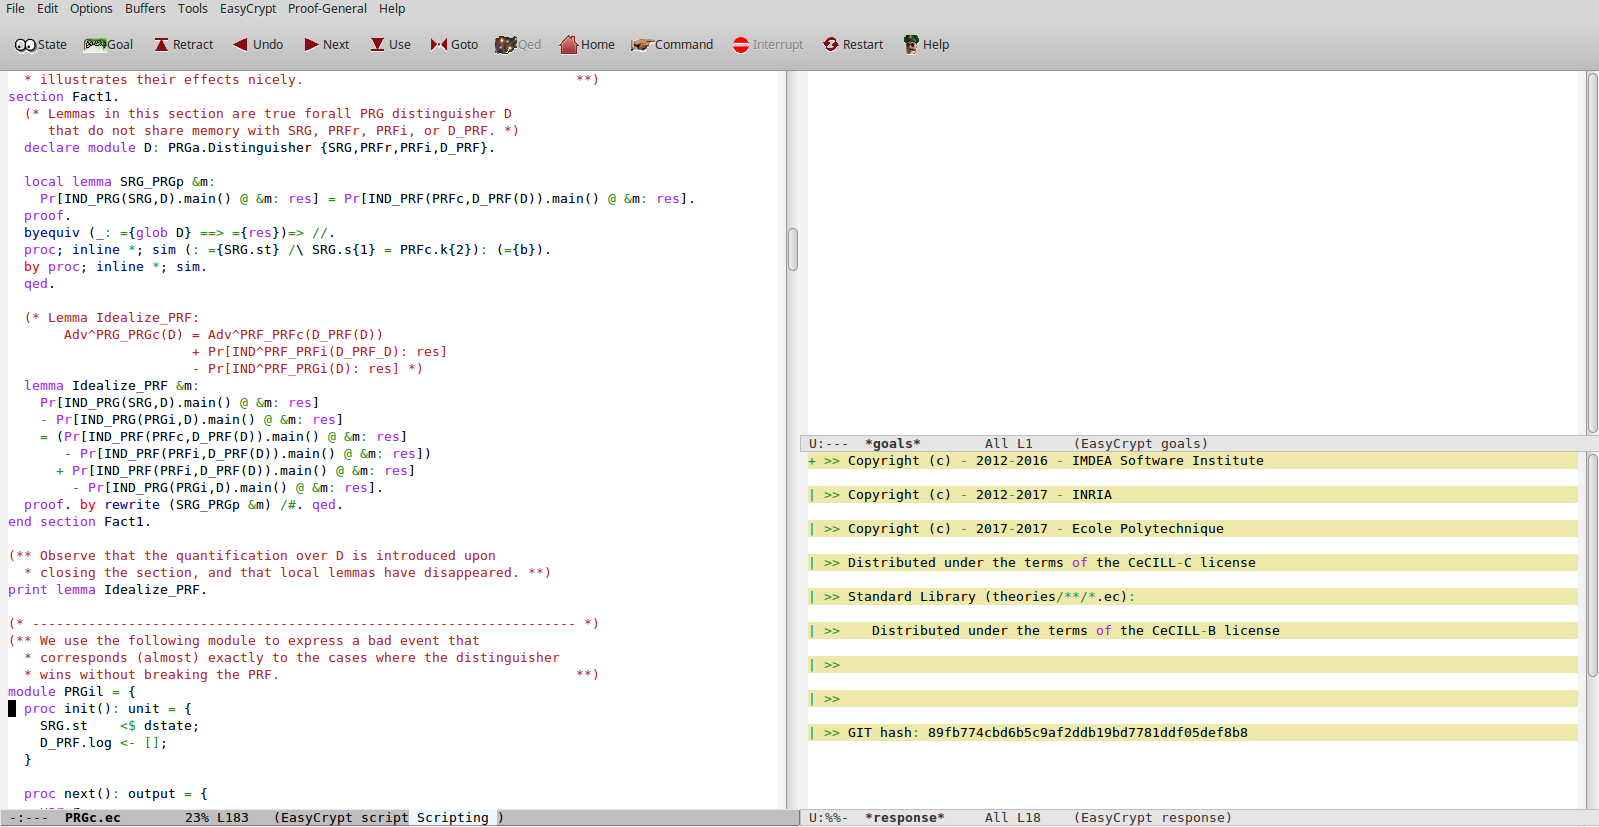
\includegraphics[width=\textwidth]{figura1.png}
\caption{Interfaz gráfica de Easycrypt} \label{fig1}
\end{figure}

\section{Comparación con otras herramientas}
Como se nombró anteriormente Easycrypt es una herramienta que se utiliza para la verificación de pruebas de seguridad de sistemas criptográficos, pero no es la única. Para saber sus limitaciones y sus extensiones se comparó con otras herramientas(CertiCrypt, Verypto).

 Para este tipo de herramienta la legibilidad del código es fundamental ya que se busca que los criptografos puedan comprenderlas y evaluarlas. Además, la sintaxis intuitiva apoya a los usuarios durante la formalización, ya que pueden enfocarse en formalizar los argumentos en lugar de que tratar de entender programas poco legibles. Todas las herramientas antes mencionadas logran buena legibilidad, pero de diferentes maneras. En EasyCrypt y CertiCrypt se utiliza un lenguaje de procedimiento imperativo en sus lógicas. Ellos modelan de cerca la idea de Bellare y Rogaway de un lenguaje con estado con oráculos como procedimientos\cite{ref_article3}. Verypto integra profundamente un lenguaje de orden superior con referencias mutables basadas en índices de Bruijn en HOL\cite{ref_article4}. La legibilidad se recupera al reflejar la sintaxis en el lenguaje de términos de HOL mediante el análisis y pretty-printing tricks.

 Otra característica importante es la expresividad, la misma tiene dos dimensiones, la sintaxis y el dominio semántico. Si bien EasyCrypt y CertiCrypt admiten distribuciones discretas de subprobabilidad y un lenguaje de procedimiento, EasyCrypt también proporciona un sistema modular para admitir la abstracción y la reutilización. Verypto provee un marco más general, ya que se basa en la teoría de medidas y, por lo tanto, admite distribuciones continuas y funciones de orden superior.

EasyCrypt es presentado como el sucesor de CertiCrypt ya que  presenta un mecanismo para compilar pruebas de CertiCrypt en EasyCrypt. Además en EasyCrypt el esfuerzo humano es menor como se ve la Cuadro 2 donde se compara CertiCrypt con EasyCrypt en varias pruebas de seguridad formalizadas en ambos sistemas. Los tiempos se miden en una Intel Core 2 Duo con 2.8GHz y 4GB de RAM sobre Mac OS X 10.6.7.


\begin{table}[H]
  \caption{Comparación de EasyCrypt con CertyCrypt}
  \label{tab:simple}
  \centering
  \begin{tabular}{ |p{3cm}|p{3cm}|p{3cm}|p{3cm}|p{3cm}|  }
 \hline
 & \multicolumn{2}{|c|}{CertiCrypt} & \multicolumn{2}{|c|}{EasyCrypt} \\\cline{2-5}

 &Lines&Time&Lines&Time\\\cline{2-5}
 \hline
 ElGamal(IND-CPA)   & 565    &45s &190 &12s \\
 Hashed ElGamal(IND-CPA)& 1255  & 1m 5s & 243  & 33s\\
 Full-Domain Hash(EF-CMA) &2035 & 5m 46s&  509 & 1m 26s\\
 Cramer-Shoup(IND-CCA)    &n/a & n/a& 1637 &5m 12s\\
 \hline
\end{tabular}
\end{table}



\section{Casos de estudio de EasyCript}
%EasyCrypt es útil en sistemas de seguridad. Estos sistemas tienen una fuerte dependencia de la criptografía para garantizar las propiedades deseadas de los mismos. Por lo tanto para que estos sistemas sean correctos (seguros) es necesario contar con una demostración de que los esquemas criptográficos utilizados por el sistema lo son. Pero estas demostraciones pueden ser propensas a errores, por lo que también deben ser probadas correctas, y este es el trabajo de EasyCript. A continuación se pasa a mostrar dos ejemplos de la utilidad e importancia de la herramienta.

\textbf{Prueba de \textbf{IND-CPA security} en Hashed Elgamal\cite{ref_article5}:}
La seguridad de hashed Elgamal puede ser reducida a la suposición de \textbf{Computational Diffie-Hellman} (CDH). Esta dice que cierto problema computacional es dificil de computar dentro de un grupo cíclico. Considere un grupo cíclico $\mathcal{G}$ de orden \textit{q}, un generador elejido aleatoriamente \textit{g}, y elementos \textit{a} y \textit{b} aleatoriamente distribuidos en $\mathbb{Z}_q$ , es difícil computar $\mathnormal{g^{ab}}$ teniendo $\mathnormal{g^{a}}$ y $\mathnormal{g^{b}}$. Esta prueba consta de 243 lineas de código y tardó 33s. Los tiempos fueron medidos en un procesador 2.8GHz Intel Core 2 Duo con 4GB de memoria RAM bajo un sistema operativo Mac OS X 10.6.7.


%\textbf{CMAC y sus variantes\cite{ref_article5}:}
%El estándar CMAC cuando fue propuesto inicialmente por Iwata y Kurosawa como OMAC1 fue acompañada por una compleja prueba de seguridad basada en juego. Se utilizo EasyCrypt para formalizar una prueba de \textit{unforgeability} para CMAC. Para esto fue necesario una mejora y extensión a la librería estándar de EasyCrypt. Además de demostrar la seguridad similar a la obtenida por Iwata y Kurosawa\cite{ref_article6} en CMAC, se probo la seguridad de construcciones intermedias como ECBC, FCBC y XCBC\cite{ref_article7}. En la siguente sección se verá con mayor detalle este caso.

\textbf{Demostración formal de CMAC y sus variantes\cite{ref_article6}:}
El estándar CMAC cuando fue propuesto inicialmente por Iwata y Kurosawa como OMAC1 fue acompañada por una compleja prueba de seguridad basada en juego. Se utilizo EasyCrypt para formalizar una prueba de \textit{unforgeability} para CMAC. Para esto fue necesario una mejora y extensión a la librería estándar de EasyCrypt. Además de demostrar la seguridad similar a la obtenida por Iwata y Kurosawa\cite{ref_article7} en CMAC, se probo la seguridad de construcciones intermedias como ECBC, FCBC y XCBC\cite{ref_article8}.

Un código de autentificación de mensajes(MAC) es una pequeña porción de información (\textit{tag}) que se agrega a un mensaje y se usa para verificar su autenticidad e integridad. Una MAC se considera segura cuando un a esquema de algoritmos generadores de \textit{tags} de MACs le resulta extremadamente difícil producir un \textit{tag} valido sin conocer la clave secreta, aun teniendo la habilidad de obtener \textit{tags} validos de mensajes específicos. CMAC es actualmente el estándar MAC, extensamente usado en la práctica. Esta basado en \textit{cypher block chaining MAC} (CBC-MAC), el cual es un esquema muy sencillo que permite la construcción de un esquema MAC para un mensaje de tamaño fijo que se restringe a partir del tamaño de bloque de un \textit{block cypher} que se asume seguro. Para sobreponerse a esta restricción se propusieron variantes de CBC-MAC llamadas ECBC, FCBC, XCBC. Sin embargo, cada uno de estos esquemas requiere una clave mas larga que la solicitada por el \textit{block cypher}. Por otra parte CMAC fue la primer variante \textit{one-key CBC-MAC}, solo usa clave de \textit{block cypher} y fue probado seguro por Iwata y Kurosawa.

Para comprender el mecanismo de CMAC es necesario entender algunos conceptos esenciales de MAC y \textit{block cypher}. Primero, un esquema MAC se compone de tres algoritmos, un algoritmo probabilistico generador de claves, que para la entrada de parámetros de seguridad devuelve una clave \textit{k} $\in$ $\mathcal{K}$ \textit{keyspace}; un algoritmo de \textit{tagging} que dado una clave y un mensaje, genera un \textit{tag}; y un algoritmo de verificación, que dado una clave, un mensaje y un \textit{tag}, devuelve un booleano que identifica si el \textit{tag} es valido para el mensaje con esa clave. Segundo, un \textit{block cypher} es una familia de permutaciones sobre un conjunto finito de bloques indexado por $\mathcal{K}$.

El esquema de demostración consiste en el uso de juegos, algoritmos probabilísticos que describen como puede interactuar un adversario con el esquema cuya seguridad se intenta vulnerar, y en que consiste dicho quiebre. Entonces la seguridad queda expresada como una propiedad de la probabilidad de que ocurra una violación de seguridad de cualquier adversario, dentro de una clase admisible de adversarios. Luego, para verificar la seguridad de CMAC se siguen una serie de pasos a través de los cuales no solo se prueba CMAC, si no también se verifica la seguridad de ECBC, FCBS, y FCBC. Ya que, si se verifica que ECBC es seguro; luego como ECBC es perfectamente indistinguible de FCBC y CMAC es computacionalmente indistinguible de FCBC; entonces se verifica la seguridad de CMAC.

\begin{description}
\item[Seguridad de ECBC:] La probabilidad en este sistema esta definida como una noción \textit{game-based}, a través de un juego de búsqueda de colisiones, en el cual al adversario $\mathcal{A}$ se le solicita una lista de mensajes de su propia elección, antes de que la función de hash \textit{h} sea aleatoriamente elegida de H, donde H es una familia de funciones hash. El adversario $\mathcal{A}$ tiene éxito si la lista de mensajes inicialmente seleccionada contiene dos mensajes distintos que tienen la misma imagen aplicados a \textit{h}.

\item[Seguridad de FCBC]: La seguridad de FCBC es equivalente a la seguridad de ECBC. Debido al hecho de que la composición de dos permutaciones aleatorias independientes se mantiene independiente de una de las permutaciones.

\item[Seguridad de CMAC]: Se relaciona la seguridad de CMAC a la de FCBC mediante el uso de las ideas de Iwata y Kurosawa en la que se plantea la indistinguibilidad de ambas. Se agrega una variable aleatoria independiente para prevenir que el adversario acceda directamente al oráculo del \textit{block cypher}.
\end{description}

\section{Conclusión}

La herramienta demuestra tener muchas ventajas sobre las alternativas existentes, ya que provee una interfaz gráfica intuitiva que permite una ejecución interactiva. También utiliza un lenguaje más expresivo y similar al formalismo de los criptógrafos, lo que resulta en la reducción del esfuerzo humano al momento de escribir el código y facilita la interpretación de las pruebas. Si bien la herramienta en sí tiene todas estos pros, existe una falencia en la distribución de la misma, ya que actualmente puede ser compleja su instalación. Por otro lado, la herramienta esta muy centrada a las necesidades de los desarrolladores, y ataca una problemática mediante métodos muy específicos.

Finalmente, EasyCript manifiesta ser uno de los framework más modernos, actualizado y confiable; al entregar robustas verificaciones.

\begin{thebibliography}{8}
\bibitem{ref_article1}
Gilles Barthe, Juan Manuel Crespo, Benjamin Gregoire, Cesar Kunz, Santiago Zanella Beguelin. Computer-Aided Cryptographic Proofs. Third International Conference, 2012.
\bibitem{ref_book1}
G. Barthe, B. Grégoire, and S. Zanella Béguelin, “Probabilistic relational hoare
logics for computer-aided security proofs,” in Mathematics of Program Construction
(J. Gibbons and P. Nogueira, eds.), vol. 7342 of Lecture Notes in
Computer Science, pp. 1–6, Springer Berlin Heidelberg, 2012.
\bibitem{ref_article2}
Gilles Barthe, Juan Manuel Crespo, Yassine Lakhnech, Benedikt Schmidt. Mind the Gap: Modular Machine-checked Proofs of One-Round Key Exchange Protocols. 34th Annual International Conference on the Theory and Applications of Cryptographic Techniques, 2015.
\bibitem{ref_article3}
Bellare, M., Rogaway, P.: The security of triple encryption and a framework for
code-based game-playing proofs. In: EUROCRYPT 2006. LNCS, vol. 4004, pp.
409–426. Springer (2006).
\bibitem{ref_article4}
Backes, M., Berg, M., Unruh, D.: A formal language for cryptographic pseudocode.
In: LPAR 2008. LNCS, vol. 5330, pp. 353–376. Springer (2008).
\bibitem{ref_article5}
Barthe G., Grégoire B., Heraud S., Béguelin S.Z. (2011) Computer-Aided Security Proofs for the Working Cryptographer. In: Rogaway P. (eds) Advances in Cryptology – CRYPTO 2011. CRYPTO 2011. Lecture Notes in Computer Science, vol 6841. Springer, Berlin, Heidelberg.
\bibitem{ref_article6}
Cécile Baritel-Ruet, François Dupressoir, Pierre-Alain Fouque and Benjamin Grégoire: Formal Security Proof of CMAC and its Variants.
31st IEEE Computer Security Foundations Symposium, 2018.
\bibitem{ref_article7}
Tetsu Iwata and Kaoru Kurosawa. OMAC: One-key CBC MAC. In FSE, volume 2887, pages 129–153. Springer, 2003.
\bibitem{ref_article8}
John Black and Phillip Rogaway. CBC MACs for arbitrary-length messages: The three-key constructions. Journal of Cryptology, 18(2):111–131, 2005.

\end{thebibliography}
\end{document}
\grid
